
%%%%%%%%%%%%%%%%%%%%%%%%%%%%%%%%%%%%%%%%%%%%%%%%%%%%%%%%%%%%%%%%%%%%%%%%%%%%%%%%%%%%%%%%%%%%%%%%%
%
% Document:      DM  SST organisation chart reporting lines
%
% Based on the DM organisation chart reporting lines by William O'Mullane
%%%%%%%%%%%%%%%%%%%%%%%%%%%%%%%%%%%%%%%%%%%%%%%%%%%%%%%%%%%%%%%%%%%%%%%%%%%%%%

\documentclass{article}

\usepackage{times,layouts}
\usepackage{tikz,hyperref,amsmath}
\usetikzlibrary{positioning,arrows,shapes,decorations.shapes,shapes.arrows}
\usetikzlibrary{backgrounds,calc}

\usepackage[paperwidth=25.5cm,paperheight=13.5cm,
left=1mm,top=5mm,bottom=0mm,right=0mm,
noheadfoot,marginparwidth=0pt,includemp=false ]{geometry}


\newcommand\showpage{%
\setlayoutscale{0.5}\setlabelfont{\tiny}\printheadingsfalse\printparametersfalse
\currentpage\pagedesign}


\hypersetup{pdftitle={DM SST organisation }, pdfsubject={Diagram illustrating the reporting lines in LSST SST DM Group},
pdfauthor={Leanne Guy}}


%%%%%%%%%%%%%%%%%%%%%%%%%%%%%%%%%%%%%%%%%%%%%%%%%%%%%%%%%%%%%%%%%%%%%%%%%%%%%%%%%%%%%%%%%%%%%%%%%
%
% Document:      Boxes and lines for all diagrams
%
%%%%%%%%%%%%%%%%%%%%%%%%%%%%%%%%%%%%%%%%%%%%%%%%%%%%%%%%%%%%%%%%%%%%%%%%%%%%%%

\tikzstyle{divbox}=[rectangle, rounded corners=3pt, draw=blue, top color=blue!30!white, bottom
color=white, very thick, minimum height=12mm, inner sep=3pt, text centered, text width=35mm]

\tikzstyle{arcbox}=[rectangle, rounded corners=3pt, draw=red, top color=yellow!50!white, bottom
color=white, very thick, minimum height=12mm, inner sep=2pt, text centered, text width=50mm]

\tikzstyle{psbox}=[rectangle, rounded corners=3pt, draw=red, top color=green!50!white, bottom
color=cyan, very thick, minimum height=10mm, inner sep=2pt, text centered, text width=35mm]

\tikzstyle{pobox}=[rectangle, rounded corners=3pt, draw=red, top color=blue!50!white, bottom
color=cyan, very thick, minimum height=10mm, inner sep=2pt, text centered, text width=35mm]

\tikzstyle{docbox}=[rectangle, rounded corners=3pt, draw=black, fill=cyan!50!white, 
 very thick, minimum height=12mm, inner sep=2pt,  text centered, text width=30mm]

\tikzstyle{docboxm}=[rectangle, rounded corners=3pt, draw=black, fill=red!50!white, 
 very thick, minimum height=12mm, inner sep=2pt,  text centered, text width=30mm]

\tikzstyle{docboxicd}=[rectangle, rounded corners=3pt, draw=black, fill=green!70!white, 
 very thick, minimum height=12mm, inner sep=2pt,  text centered, text width=30mm]

\tikzstyle{gbox}=[rectangle, rounded corners=3pt, draw=orange!80!black, top color=orange!30!white,
bottom color=white, very thick, minimum height=12mm, inner sep=5pt, text badly ragged, text width=40mm]

\tikzstyle{mbox}=[rectangle, rounded corners=3pt, draw=blue, top color=cyan!50!white, bottom
color=white, very thick, minimum height=8mm, inner sep=2pt, text centered, text width=30mm]

\tikzstyle{line}=[-, thick]
\tikzstyle{sline}=[-, thick, dashed, olive]
\tikzstyle{dline}=[->, thick, cyan]
\tikzstyle{tline}=[->, thick, dashed, blue]
\tikzstyle{pline}=[->, thick,  black!60!white]

\xdefinecolor{softviolet}{rgb}{0.85, 0.8, 1.0}




\begin{document}

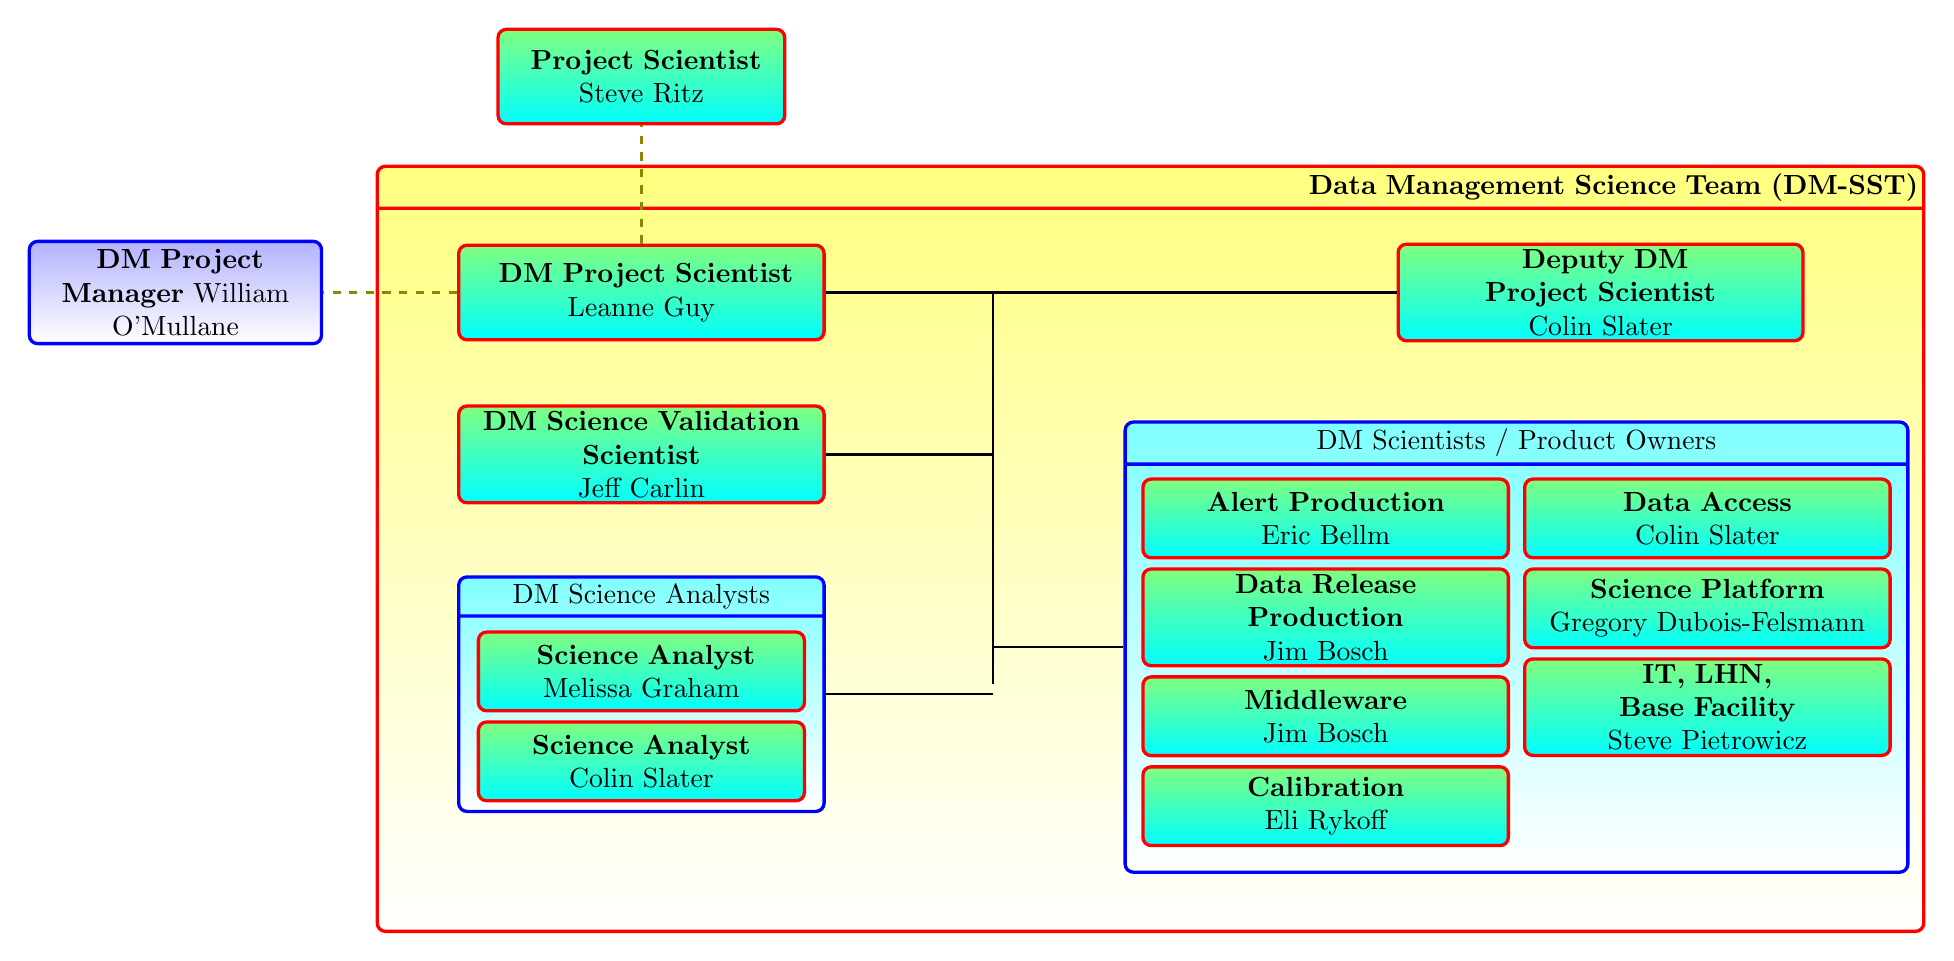
\begin{tikzpicture}[node distance=0mm]


    \node (dm) [arcbox, align=right, text width=19.5cm,  minimum height=13mm, rectangle split, rectangle split parts=2]
    { \hspace{0.1cm} \textbf{Data Management  Science Team (DM-SST)}
	   \nodepart{second} \vspace{90mm}
	};

    \node (dmpsanc) [below=1.5cm of dm.north]{};   
    \node (dmps) [psbox, left=4.0cm of dmpsanc, minimum height=12mm, text width=45mm] {\textbf{ DM Project Scientist}\\ Leanne Guy };
    \node (ddmps) [psbox, right=3.0cm of dmpsanc, minimum height=12mm, text width=50mm] {\textbf{ Deputy DM Project Scientist}\\ Colin Slater };
    \node (ps) [psbox, above=1.5cm of dmps, minimum height=12mm] {\textbf{  Project Scientist}\\ Steve Ritz};
     \node (dmpm) [divbox, left=1.7cm of dmps] {\textbf{ DM Project Manager} William O'Mullane};

 
% Validation Scientist
    \node (valsci) [psbox, below=8mm of dmps.south , text width=45mm, minimum height=12mm] {\textbf{DM Science Validation \\Scientist}\\  Jeff Carlin};

   
 %SST  analysts
            \node (sstanal) [mbox, text width=45mm, rectangle split, rectangle split parts=2, below=9mm of valsci ]
                {
                DM Science  Analysts
                \nodepart{second} \vspace{23mm}
                };
    \node (sstanal-mlg) [psbox, below=7mm of sstanal.north, text width=40mm] {\textbf{ Science Analyst }\\ Melissa Graham };
    \node (sstanal-cts) [psbox, below=1mm of sstanal-mlg, text width=40mm] {\textbf{Science Analyst}\\ Colin Slater};
%
% Institutional Science Leads
           \node (upo) [right=14mm of ddmps.west, text width=0mm]{};
            \node (instleads) [mbox, text width=98mm, rectangle split, rectangle split parts=2,  below= 15mm of upo]
                {
                DM Scientists / Product Owners
                \nodepart{second} \vspace{50mm}
                };
    \node (upo1) [left=23mm of instleads.north, text width=0mm]{};
    %\node (pipesci) [psbox, below=6mm of upo1, text width=45mm] {\textbf{Science Pipelines }\\ Jim Bosch};
    \node (apsc) [psbox, below=6mm of upo1, text width=45mm] {\textbf{Alert Production }\\ Eric Bellm };
    \node (drpsc) [psbox, below=1mm of apsc, text width=45mm] {\textbf{Data Release \\Production}\\ Jim Bosch};
    \node (calsci) [psbox, below =1mm of drpsc, text width=45mm] {\textbf{Middleware }\\ Jim Bosch};
    \node (suitsc) [psbox, below=1mm of calsci, text width=45mm]  {\textbf{Calibration }\\ Eli Rykoff};


      
    \node (upo2) [right=23mm of instleads.north, text width=0mm]{};
    \node (dfsc) [psbox, below=6mm of upo2, text width=45mm] {\textbf{Data Access  }\\ Colin Slater};
    \node (nwsc) [psbox, below=1mm of dfsc, text width=45mm] {\textbf{Science Platform }\\ Gregory Dubois-Felsmann};
   \node (mwsc) [psbox, below=1mm of nwsc, text width=45mm] {\textbf{IT, LHN, \\Base Facility  }\\  Steve Pietrowicz  };
     % \node (daxsc) [psbox, below=1mm of mwsc, text width=45mm] {\textbf{Data Facility }\\  Leanne Guy }; 
  %  \node (sqsc) [psbox, below=1mm of daxsc, text width=45mm] {\textbf{Software Quality (SQuaRE) }\\  Leanne Guy };


%%%% Legend
%%\node (leg) [lbox, below=4cm of admin, text width=35mm,  minimum height=10mm, rectangle split, rectangle split parts=2]
%%    { \hspace{0.1cm} \textbf{Legend}
%%           \nodepart{second} \vspace{30mm}
%%        };
% %\node(snode) [psbox,below=0.7cm of leg.north, text width=30mm] {Science Role};
% %\node(pnode) [mbox,below=0.1cm of snode, text width=30mm] {Technical Role};
% %\node(mnode) [mbox,below=0.1cm of pnode, text width=30mm] {Managment/other Role};
%
\draw[sline] (dmps.north) --  (ps.south);
 \draw[sline] (dmps.west) --  (dmpm.east);
  \draw[line] (dmps.east) -- (ddmps.west);

 \node (udmpm) [right=20mm of dmps, text width=0mm]{};
 \node (anc1) [right=20mm of sstanal, text width=0mm]{};
 
  \draw[line] (udmpm)  -| (anc1);  
  \draw[line] (sstanal.east) -| (anc1);  
  \draw[line] (instleads.west) -| (anc1);  
 
 \node (anc2) [right=20mm of valsci, text width=0mm]{};
 \draw[line] (valsci.east) -| (anc2);  


\end{tikzpicture}
\end{document}
